\documentclass[spanish]{article}
\usepackage[spanish]{babel}
\usepackage{amsmath}
\usepackage{amssymb}
\usepackage[utf8]{inputenc}
\usepackage{vmargin}
\usepackage{graphicx}
\usepackage{wrapfig}
\usepackage[export]{adjustbox}


\begin{document}
	\setpapersize{USletter}
	\setmarginsrb{30mm}{30mm}{30mm}{30mm}{0pt}{0mm}{0pt}{0mm}
	
	\begin{center}
	{ Análisis de Algoritmos, Sem: 2018-1, 3CV2 Práctica 7, 2 de Noviembre del 2017}\\
{ {\bf Práctica 7: Multiplicacion de una secuencia de matrices}} \\
{ {\bf Martínez Berumen Luis Daniel}} \\

\includegraphics[width=1\textwidth, right]{./imagenes/logos.png}
	\end{center}

	\bigskip
	
	\bigskip
	
	\bigskip
	
	{\LARGE {\bf Abstract}}\\
En esta Practica analizaremos la complejidad del algoritmo de la multiplicacion secuencial de matrices, así como demostraremos su funcionamiento, daremos un ejemplo de como funciona con matrices aleatorias.

\bigskip

	{\Large {\bf Palabras Clave}}\\
	\begin{itemize}
		\item Algoritmo
		\item Complejidad
		\item Multiplicación
		\item Secuencia
		\item Dinámica
	\end{itemize}
	
	\section{Introducci\'on}
Divide y Vencerás es una frase quye hemos escuchado todos, al menos, una vez en nuestra vida, para nosotros 
	es técnica de diseño de algoritmos, siendo de gran utilidad para nuestra carrera, ya que, 
	los problemas a los que nos enfrentamos día con día son mas faciles de resolver si aplciamos una tecnica de este tipo.
	De hecho, suele ser considerada una filosofía general para resolver problemas, no solo del termino informatico, sino que también           se utiliza en muchos otros ámbitos

\newpage

	\section{Conceptos B\'asicos}
	Para la correcta comprension de este trabajo, es necesario definir algunos terminos tales como $\theta$, O y $\Omega$.\\
	 $\theta$(n):\\
		Sea g(n) una función. Se define  $\theta$ (g(n)) como:\\
		
		 	$\theta$(g(n)) = $\{ f(n) \quad | \quad \exists c1,c2>0 \quad \& \quad n_{0}>0 \quad \mid \quad \forall n>=n_{0} \quad 0<= c1g(n) <= f(n) <= c2g(n) \}$
	\bigskip		 	
		 	
	O(n):\\
		Sea  g(n)  una función, O(n) (el pero de los casos) se define como:\\
		
			\hspace{1cm}O(n)=$\{f(n) \quad | \quad \exists c >0 \quad \& \quad n_{0}>0 \quad | \quad f(n) <= Cg(n) \quad \forall  n>= n_{0} \}$
	\bigskip
	
	$\Omega$(n):\\
	Sea  g(n)  una función. Se define $\Omega$ (g(n)) (el mejor de los casos) como:\\

		\hspace{1cm}$\Omega$(g(n)) =$\{f(n) \quad | \quad \exists c >0 \quad \& \quad n_{0}>0 \quad \mid \quad  0<= cg(n)<= f(n) \quad \forall n>= n_{0} \}$
	\bigskip

	Dentro del trabajo solo se observará la ejecución del algoritmo de  multiplicación secuencial de matrices, corroborando la salida del programa, con el resultado esperado, posteriormente se planteará la demostraciñon de la función que rige el algoritmo.


		
	\newpage


\section{Experimentaci\'on y Resultados}

	\subsection{ 1 Implementar el algoritmo de  multiplicación secuencial de matrices}
	
	{\large{ {\bf i) Como entrada el algoritmo tendrá n matrices $A_{i}$ de tamaño $p_{i-1}$ X $p_{i}$.}}}\\
	\begin{center}
		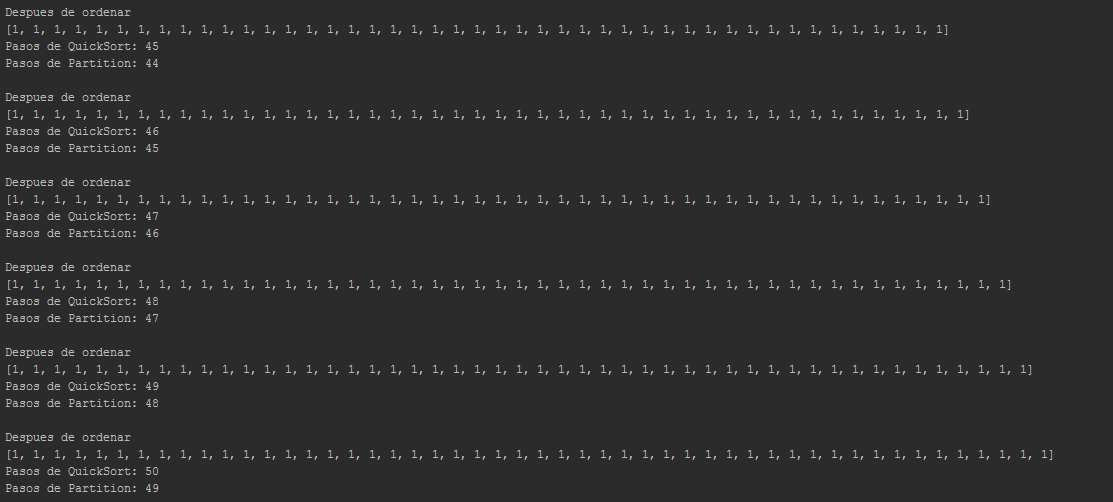
\includegraphics[width=0.60\textwidth]{./imagenes/1.png}\\
		Figura 1. Entrada de 5 matrices.\\
	\end{center}
	${\bf Entrada:}$ 3,5,6,5,3,3 (Hace referencia implícitamente a cinco matrices $A_{i}$ = $A_{3x5}$ , $A_{2}= A_{5x6}$, $A_{3}=A_{6x5}$,$A_{4}=A_{5x3}$, $A_{5}=A_{3x3}$).\\

{\large{\bf ii)  Como salida, se mostrará la configuración de paréntesis que genera el algoritmo.}}\\
	\begin{center}
		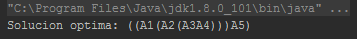
\includegraphics[width=0.60\textwidth]{./imagenes/2.png}\\
		Figura 2. <<Parentizacion>> optima para las 5 matrices.\\
	\end{center}
\newpage	
	{\large{\bf iii)Además se mostrarán todas las configuraciones de paréntesis y se corroborará que la generada en el punto ii) en efecto, es la óptima .}}\\

\begin{center}
		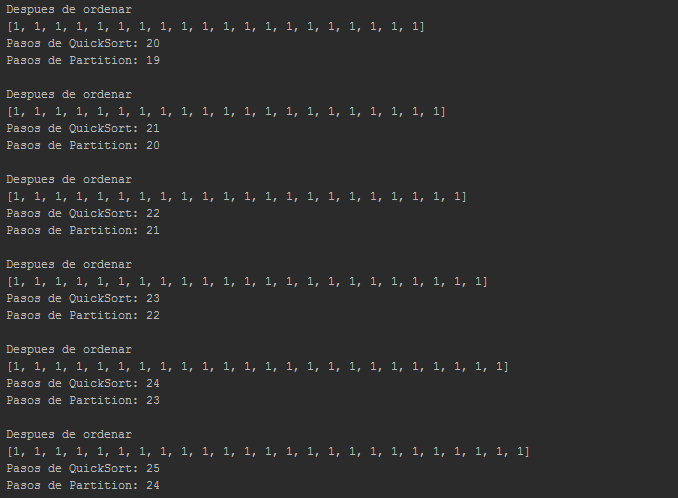
\includegraphics[scale=.75]{./imagenes/3.png}\\
		Figura 3. Todas las configuraciones.\\
	\end{center}
	


	Ejemplo.
	${\bf Entrada:}$ 3,5,2,2 (Hace referencia implícitamente a tres matrices $A_{i}$ = $A_{3x5}$ , $A_{2}= A_{5x2},A_{3}=A_{2x2}$).\\
	${\bf Salida:}$ \\
	La configuración que genera el algoritmo de multiplicación de una secuencia de matrices es: $((A_{1}A_{2})A{3})$.\\
	Muestra todas las configuraciones y las operaciones escalares realizadas.\\
	$(A_{1}(A_{2}A_{3}))$ realiza 20 operaciones escalares\\
	$((A_{1}A_{2})A_{3})$ realiza 42 operaciones escalares\\
	Por lo tanto una configuración óptima es $((A_{1}A_{2})A_{3})$.\\
\newpage
	
	\section{Conclusi\'on}

	La ideología de divide y vencerás hace el problema más mas sencillo de analizar, pero no siempre se está seguro que la solución presentada sea la más óptima.\\
	Es importante dejar claro que el analisis de algoritmos es una parte muy importante de la carrera, ya que los vamos a utilizar SIEMPRE, dicho esto es importante recalcar que no todos los algoritmos pueden ser la mejor opcion.\\
	Por eso es fundamental saber obtener los mejores resultados para simplificar tareas grandes, obteniendo así un ahorro tanto en tiempo como en recursos.
		
\section{Anexos}
${\bf Problema :}$ Utilizando método por sustitución muestre que la ecuación de recurrencia P(n)= $\sum_{i=0}^{n-1}P(K)P(n-k)$ si n>=2 y P(n=1)=1 cumple con la definición 1.5 $\Omega$ ($2^{n}$ 

	\section{Bibliografía}
	\begin{itemize}
		\item Brassard, G. (1997). Fundamentos de Algoritmia. España: Ed. Prentice Hall. ISBN 		848966000X
		\item Harel, D. (2004). Algorithmics: The spirit of Computing (3rd. Ed). Estados Unidos de América: Addison
Wesley. ISBN-13: 978-0321117847
	\end{itemize}
	
\end{document}